\section{Import Input data}
Taking advantage of \scipion software framework, we are going to import the above indicated input data using protocols \scommand{import volumes} and  \scommand{import sequence}. Details about the parameters of these two protocols are shown in Appendices \ref{app:importVolume} and \ref{app:importSequence}, respectively. 

 \begin{figure}[H]
  \centering 
  \captionsetup{width=.9\linewidth} 
  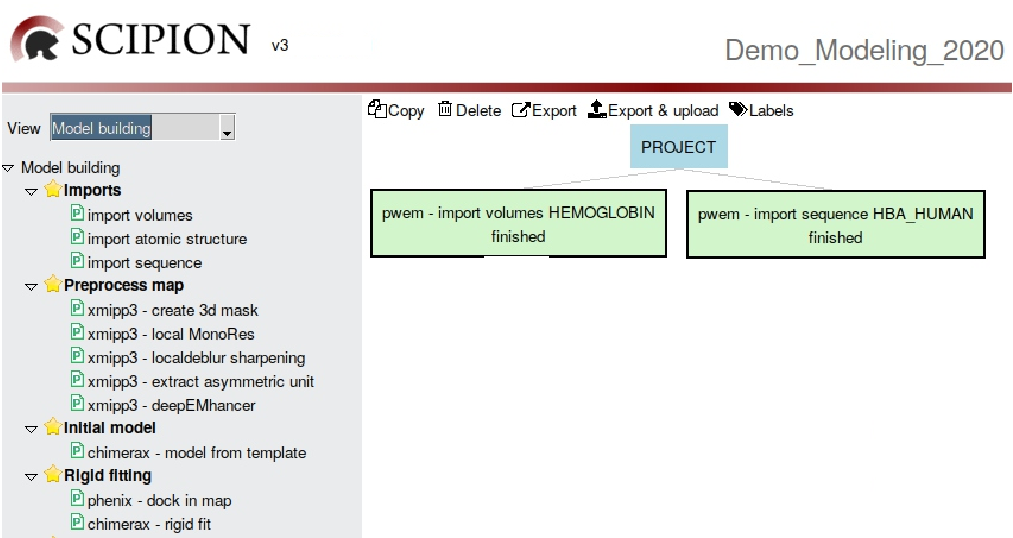
\includegraphics[width=0.95\textwidth]
  {Images/Fig61}
  \caption{\scipion framework with import workflow.}
  \label{fig:scipion_workflow_import_1}
  \end{figure}

(Note: The notation \ttt{Fig. X (a)} means that the step is shown in figure number X and there will be an arrow labeled with ``a'' marking the region of interest.)

 \subsection*{Volume}
 First open the \scommand{import volumes} protocol (\ffigure{fig:import_volume} (1)), fill in the form and execute it (2), and finally you may visualize the volume (3). 
 
 As you can see, when we import a map we directly assign its sampling rate and its origin of coordinates. If for any reason we have to work with other maps previously generated during the reconstruction process that do not have the desired sampling and origin, we can use the auxiliar protocol \scommand{assign Orig \& Sampling}, detailed in Appendix \ref{app:asignOrigAndSampling}, to assign them.
 
 \begin{figure}[H]
  \centering 
  \captionsetup{width=.9\linewidth} 
  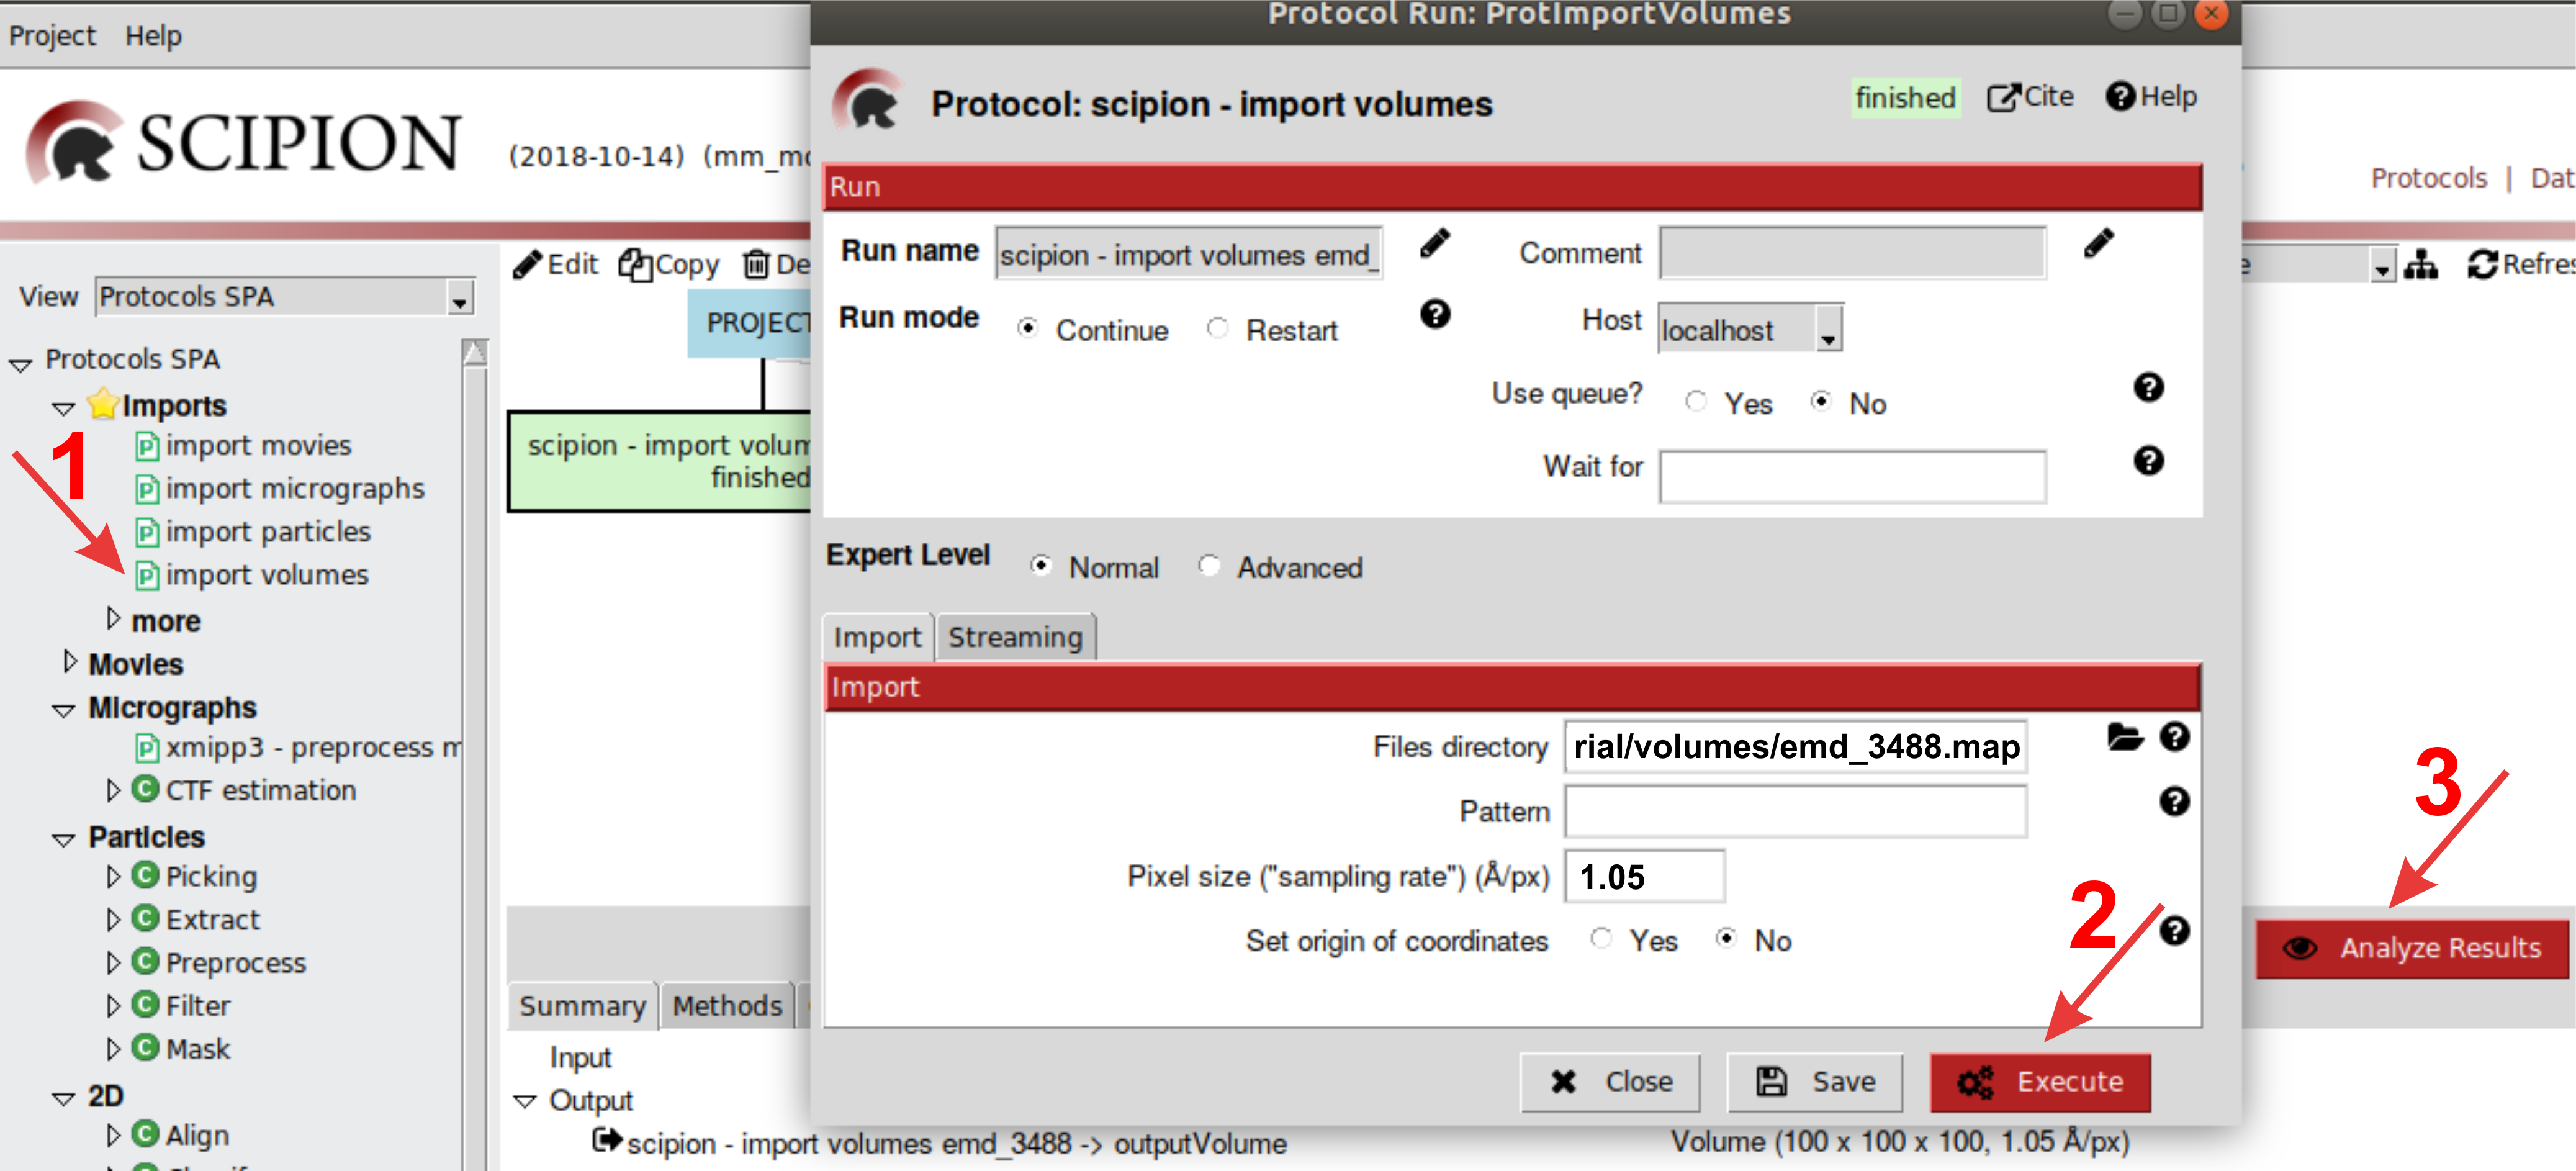
\includegraphics[width=0.95\textwidth]
  {Images/Fig4}
  \caption{Importing the volume in \scipion.}
  \label{fig:import_volume}
  \end{figure}
  
By default \chimera \citep{Goddard2018} is used for visualization. Clicking in the viewer menu  (\ffigure{fig:chimera_visualization_volume} (1)), \chimera shows the 3D map and the $x$ (red), $y$ (yellow) and $z$ (blue) axes.  
 %  The C2 symmetry is shown, as well as the 45º turn of volume regarding the z axis (blue line).
  
 \begin{figure}[H]
  \centering 
  \captionsetup{width=.9\linewidth} 
  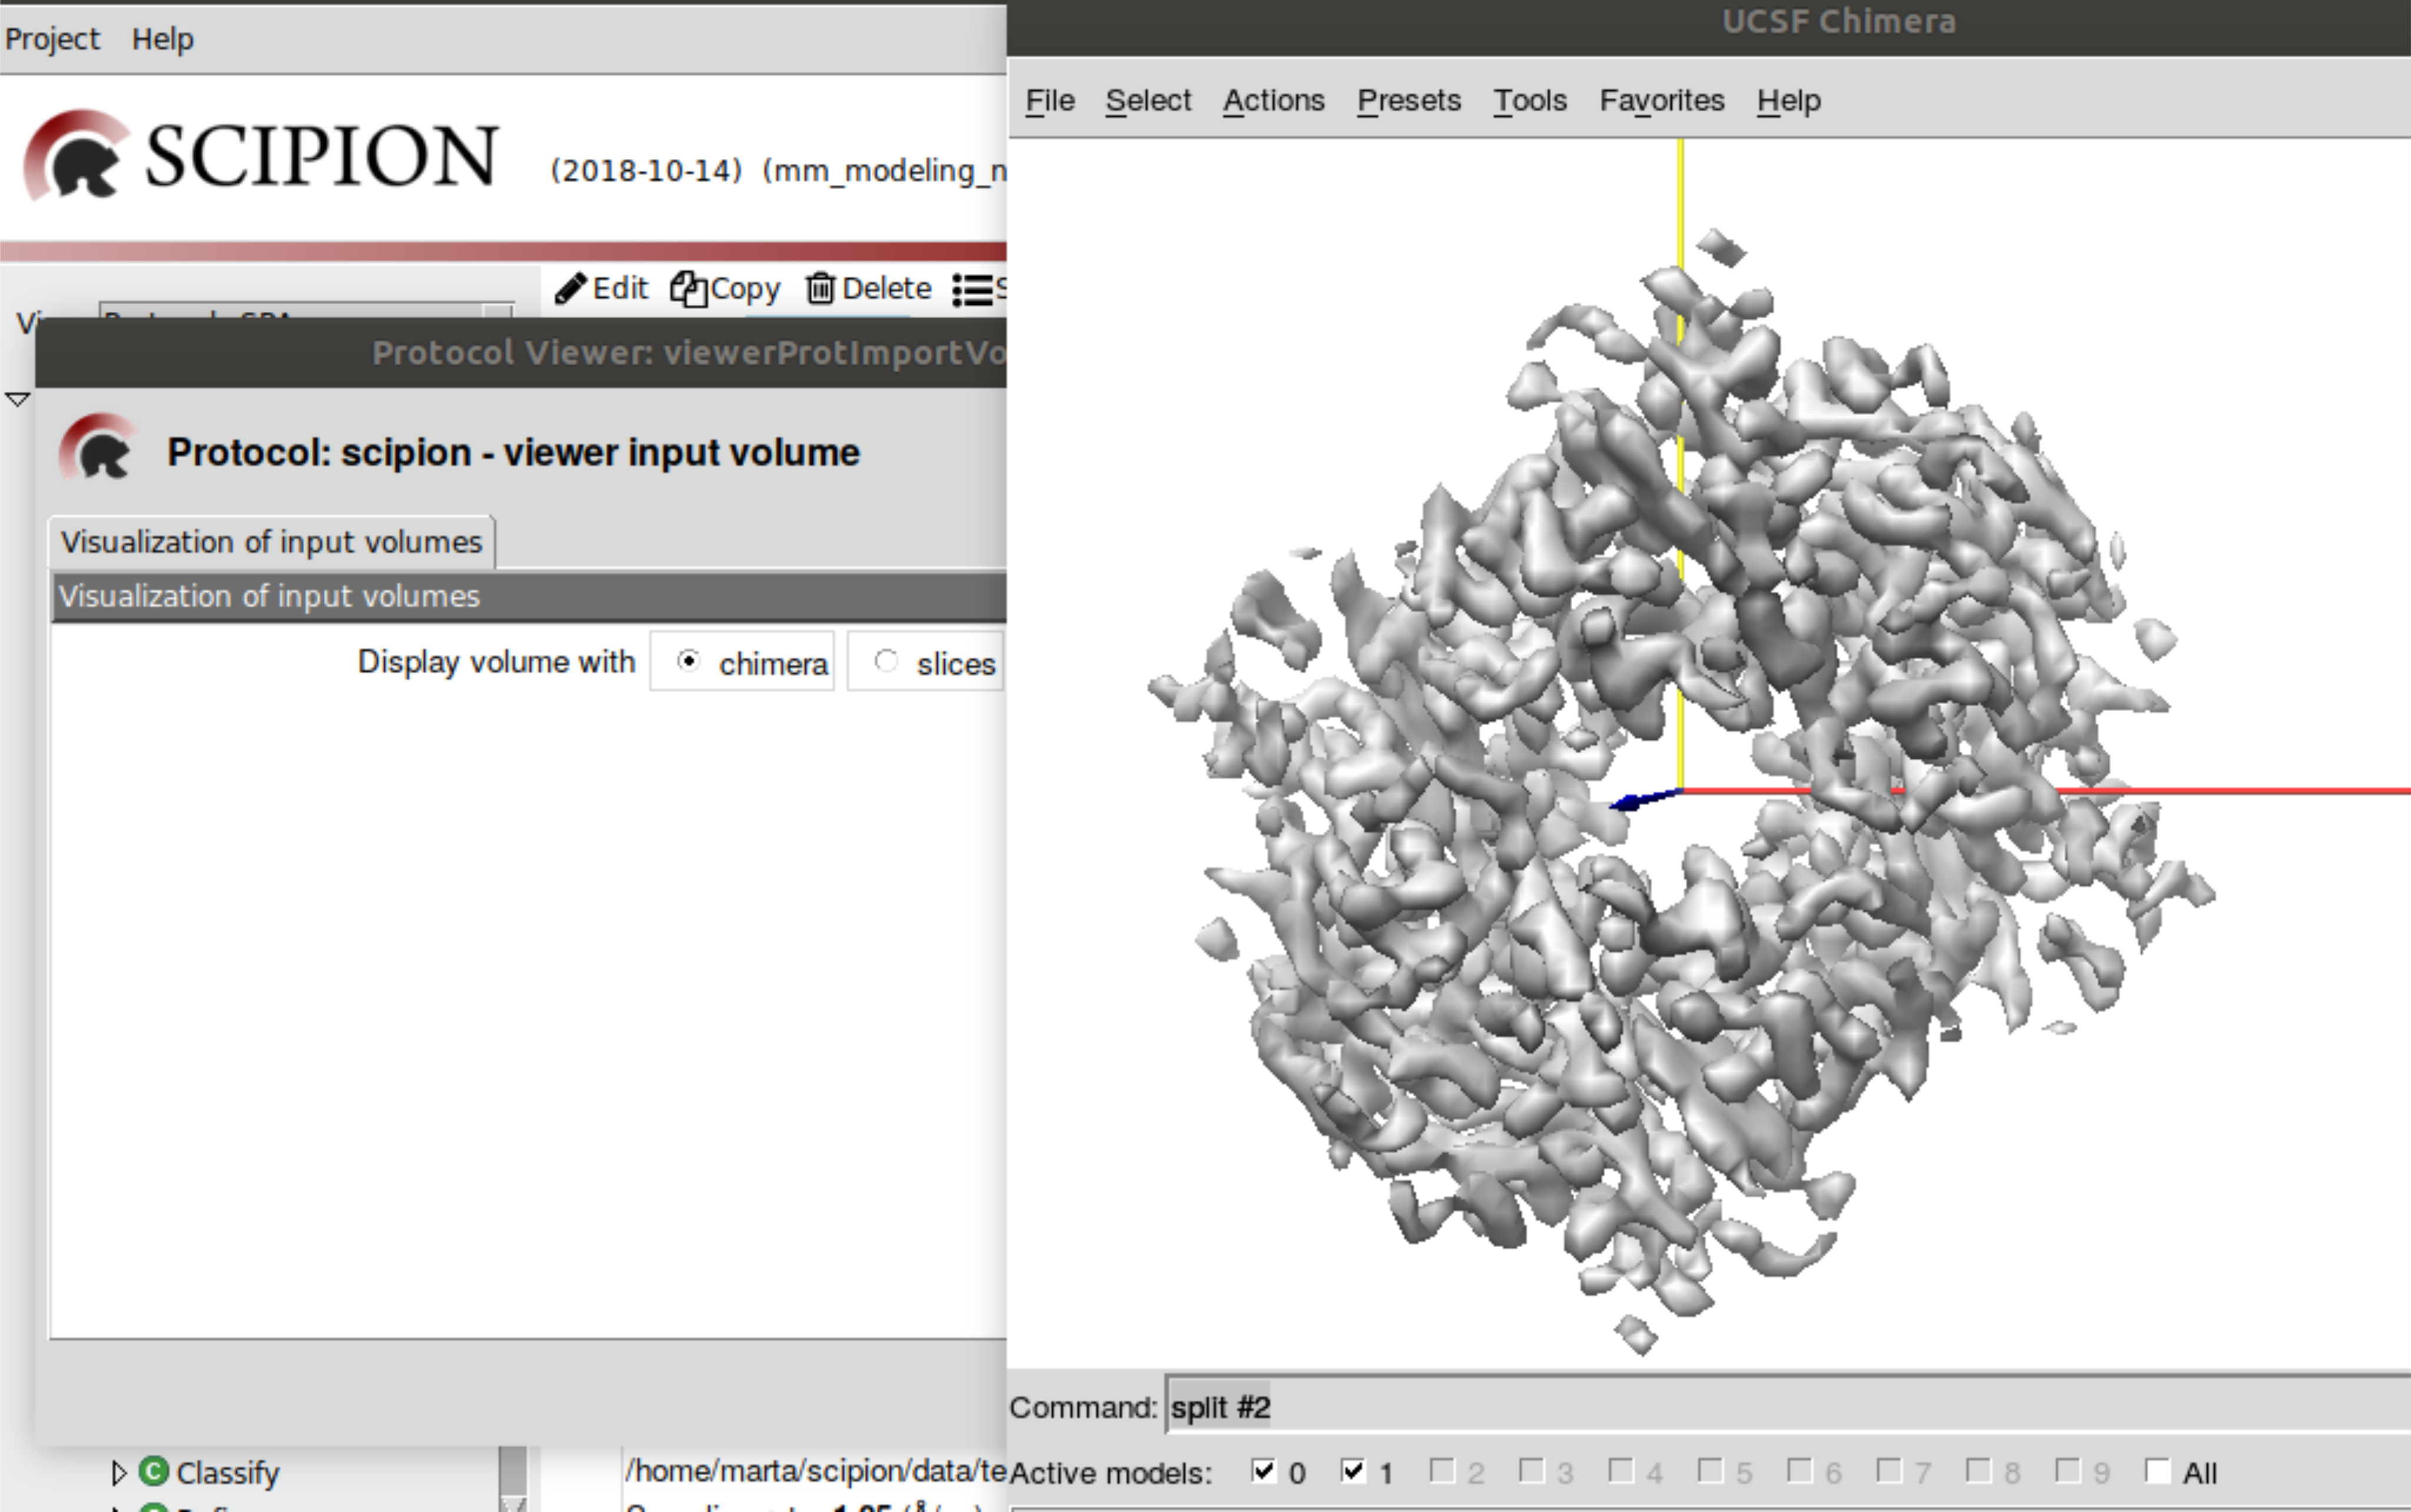
\includegraphics[width=0.95\textwidth]
  {Images/Fig5}
  \caption{Volume visualized with \chimera.}
  \label{fig:chimera_visualization_volume}
  \end{figure}
 
 \subsection*{Sequences}
 
 The sequences of \ttt{Hgb} $\alpha$ and $\beta$ subunits will be independently downloaded from \ttt{UniprotKB}. First of all, open the form of \scommand{import sequence} protocol (\ffigure{fig:import_sequence} (1)), then complete the form to download \ttt{HBA\_HUMAN} protein with \ttt{UniProtKB} accession code \ttt{P69905}, execute the process (2), and finally visualize the sequence (3) in a text editor. The sequence will appear in \ttt{fasta} format as it has been written above. Follow the same protocol to download \ttt{HBB\_HUMAN} with accession code \ttt{P68871}.
 
 \begin{figure}[H]
  \centering 
  \captionsetup{width=.9\linewidth} 
  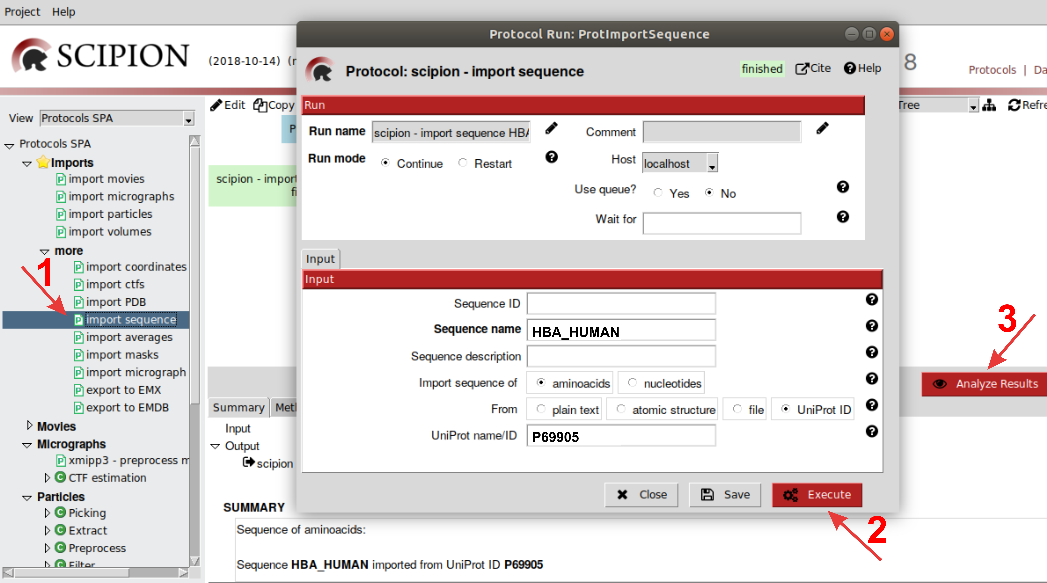
\includegraphics[width=0.95\textwidth]
  {Images/Fig6}
  \caption{Importing a \ttt{UniProtKB} sequence in \scipion.}
  \label{fig:import_sequence}
  \end{figure}
 
